\documentclass[10pt,a4paper]{article}
\usepackage[latin1]{inputenc}
\usepackage{amsmath}
\usepackage{amsfonts}
\usepackage{amssymb}
\usepackage{graphicx}
\usepackage{pdfpages}

\author{Bhavya Joshi \& Florian J�rg}
\title{Fundamentals of Simulation methods\\\Large{Solution Sheet 4}}
\begin{document}
	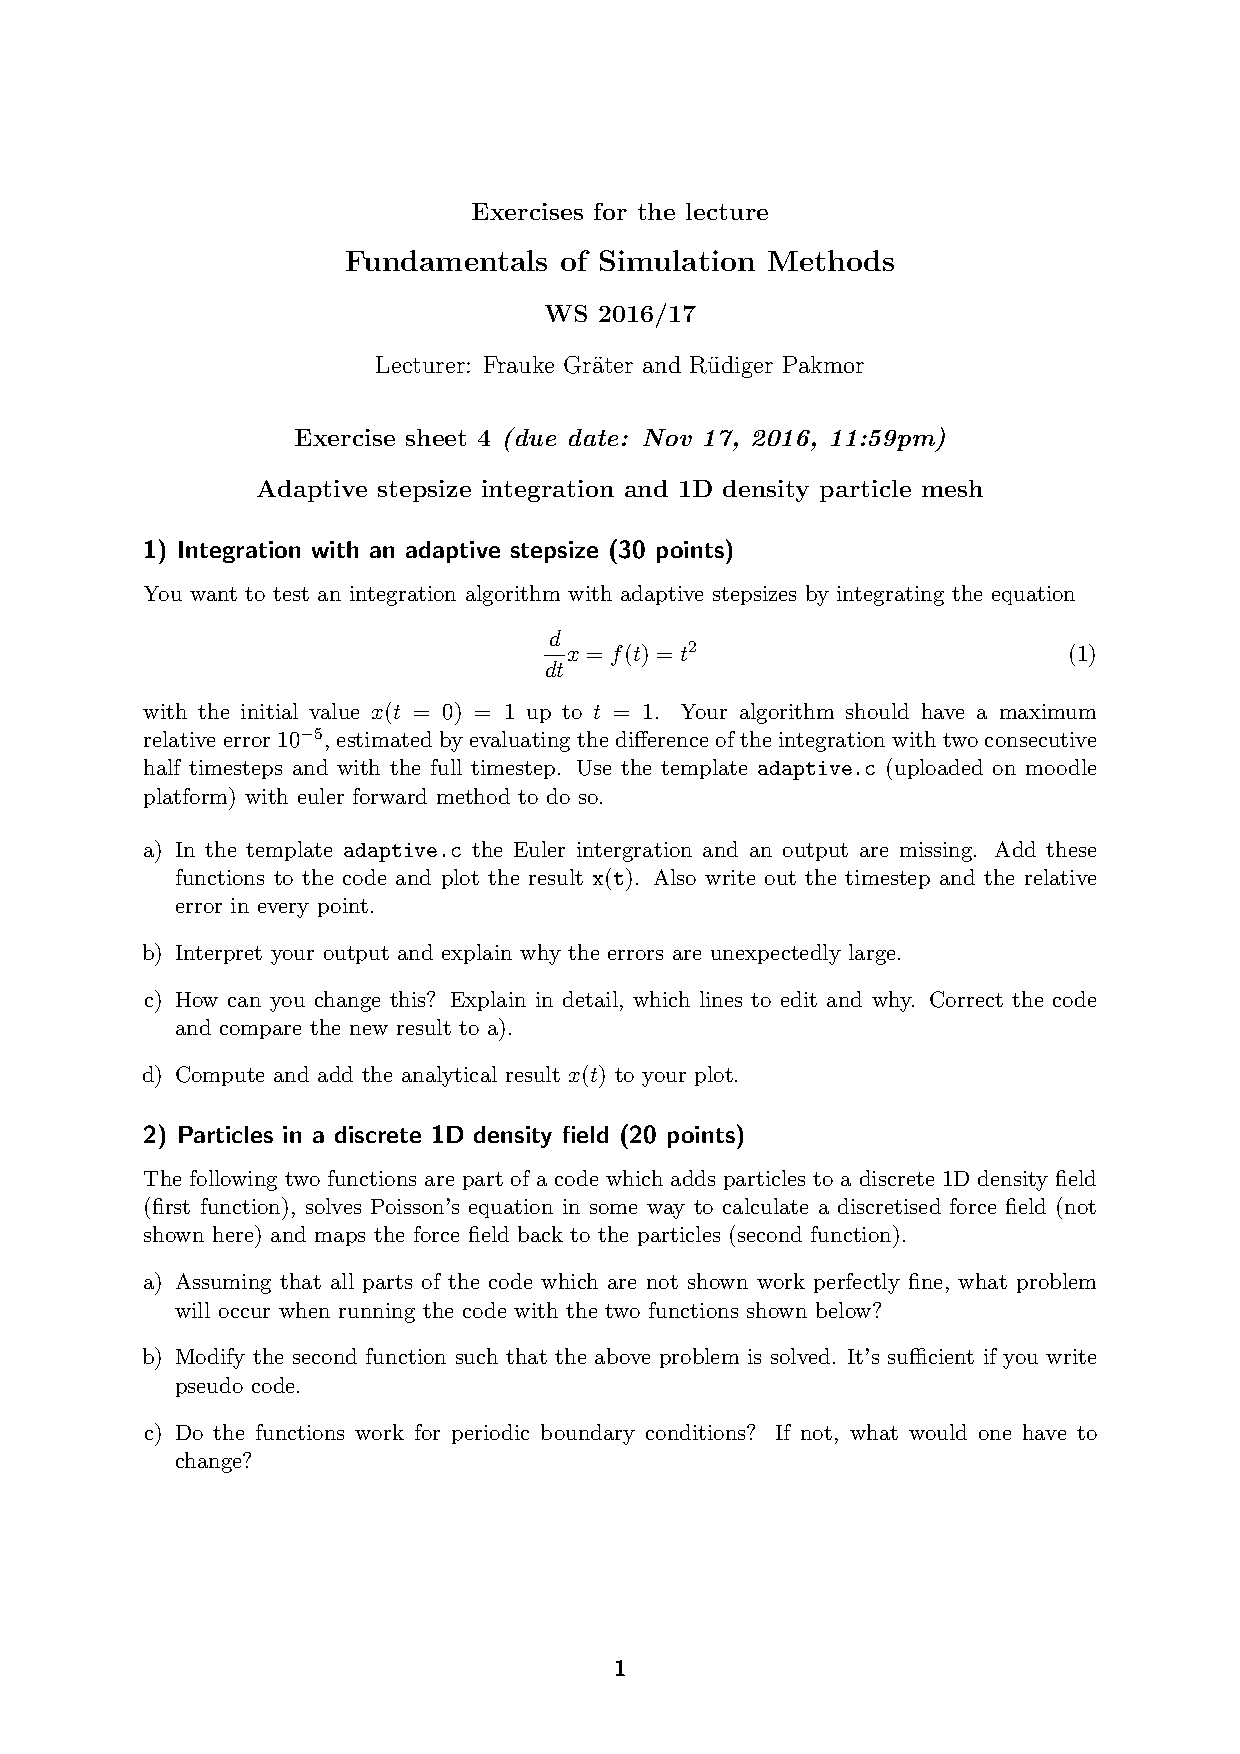
\includepdf[pages=-]{exercise4.pdf} 
	\maketitle
	\section*{Exercise 1:}
	
\subsection*{a)}

After modification of the given script, we get the results given in table \ref{tab:ex1_a}.

\begin{table}[h]
	\caption{??}\label{tab:ex1_a}
	\centering
	\begin{tabular}{lllll}
		\hline\hline
time& $x_{Euler}$& $\Delta t$& absolute error& $x_{ana}$\\
\hline
0& 1& 0.5& 0 & 1\\
0.5& 1.01562& 0.25& 0.015625& 1.04167\\
0.75& 1.0957& 0.125& 0.0175781& 1.14062\\
0.875& 1.17212& 0.0625& 0.00610352& 1.22331\\
0.9375& 1.22171& 0.03125& 0.0017395& 1.27466\\
0.96875& 1.24964& 0.015625& 0.000461578& 1.30305\\
0.984375& 1.26442& 0.0078125& 0.000118732& 1.31795\\
0.992188& 1.27202& 0.00390625& 3.01003e-05& 1.32558\\
0.996094& 1.27587& 0.00390625& 7.57724e-06& 1.32944\\
1& 1.27976& 0.00390625& 7.60704e-06& 1.33333\\
\hline\hline		
	\end{tabular}
\end{table}

\subsection*{b)}
{\color{red}Interpretation of the outputs!}
	
\subsection*{c)}
{\color{red}Solution to the big errors?!}

\subsection*{d)}

The analytical solution follows from the integration using separation of variables and is given by

\begin{align}
	&\frac{d}{dt}x = t^2\nonumber\\
	\Rightarrow\qquad &\int  dx = \int t^2 dt\nonumber\\
	\Rightarrow\qquad & x(t) = \frac{1}{3}t^3 + c\nonumber
\end{align}
The integration constant $c$ can be computed by using the condition that the given initial value $x(t = 0) = 1$ must be met. Therefore $c = 1$. And the analytical solution is given by
\begin{align}
	x(t) = \frac{1}{3}t^3 + 1\label{eq:ex1_analytical}
\end{align}

Figure \ref{fig:ex1_d} shows the solution computed using the forward Euler Method together with the analytical solution given in equation \ref{eq:ex1_analytical}.
	\begin{figure}[h]
		\centering
		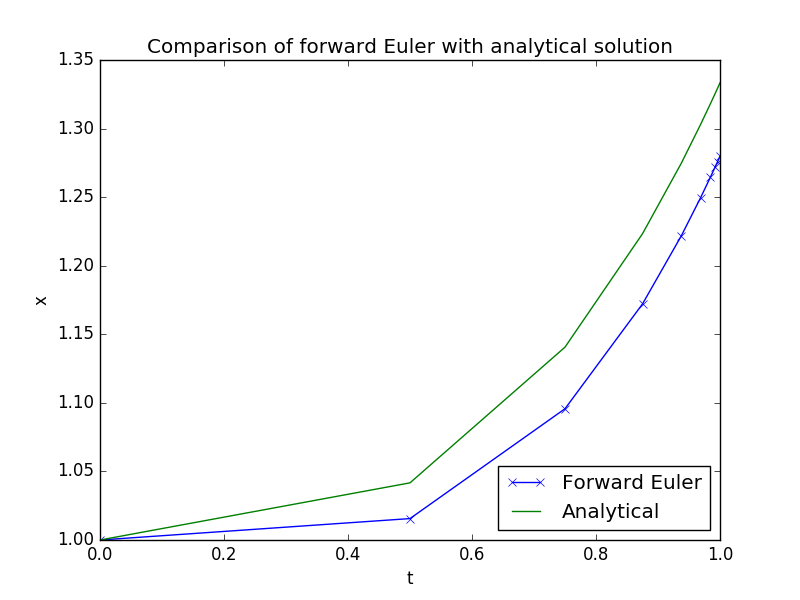
\includegraphics[width=\textwidth]{fig_1_d.png}
		\caption{Comparison of the result of forward Euler method and analytical solution}\label{fig:ex1_d}
	\end{figure}

\section*{Exercise 2:}

\subsection*{a)}

First - The first fuction is not returning the any value.\\
Second - The value of variable \textbf{xx} provided here will not fulfill our aim behind the calculations.\\
Third - In second fuction accelaration did not find the right way. 
 
\subsection*{b)}
Correction is submitted in the first equation program named $ex42.c$

\subsection*{c)}
 For first fuction it works for periodic boudary condition, but for second fuction it will not work for boundary condition. 

\section{Solution_class exercise_2}
we want to assign a mass to the grid point of the 1D grid. \\
So in given example, for position 5.9, we want to assign 10 percetage of mass to grid 5 
and 90 percent of mass to gird 6. 
\end{document}